\chapter{Technical Background}
\label{chap:04_background}

This chapter introduces the technologies and algorithms used for this thesis work. It explains the fundamental concepts as well as installation requirements if needed.

% ===========================================
% ===========================================
% Docker
% ===========================================
% ===========================================
\section{Docker}
\label{sec:04_docker}
% Short docker intro
Docker is an open-source platform that enables containerization of applications. Containerization is a technology to package, ship and run applications and their environment in individual containers.
% Make clear
Docker is not a container technology itself. It hides the complexity of working with container technologies directly and instead provides an abstraction and the tools to work with containers \cite{Nickoloff2019Docker, Bullington2020Docker, Potdar2020Docker}.


\subsection{Docker Architecture}
\label{subsec:04_docker_architecture}
% Architecture figure
\begin{figure}[h]
\centering
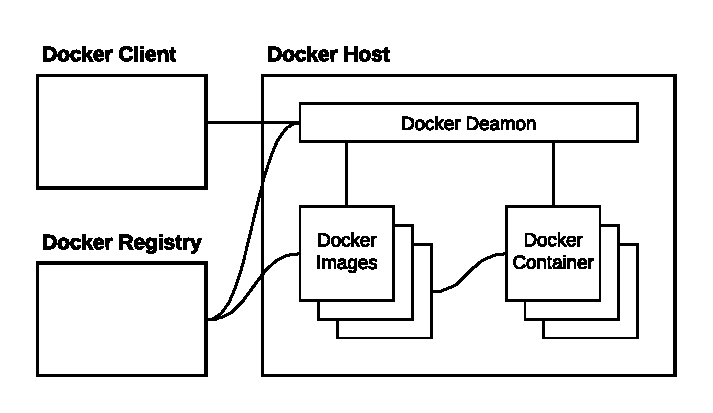
\includegraphics[scale=1]{images/04_technical_background/docker/docker_architecture}
\caption{Docker architecture - Source: Authors own model, based on \cite{Docker2020Docs}.}
\label{fig:04_docker_architecture_architecture}
\end{figure}

% Explain figure
\Fig{fig:04_docker_architecture_architecture} illustrates the client server architecture of Docker. It consists of a Docker Client, the Docker Deamon, and a Docker Registry.


\paragraph{Docker Client:} The Docker client is an interface for the user to send commands to the Docker deamon \cite{Docker2020Docs}.


\paragraph{Docker Deamon:} The Docker deamon manages all containers running on the host system and handles the containers resources, networks and volumes \cite{Bullington2020Docker}.


\paragraph{Docker Registry:} A Docker registry stores images. Images can be pushed to a public or private registry and pulled from it to build a container \cite{Docker2020Docs}.


\subsection{Docker Image}
\label{subsec:04_docker_image}
% What is an image
An Image is a snapshot of the environment that is needed to run an application in a Docker container. The environment consists of all files, libraries and configurations that are needed for the application to run properly \cite{Docker2020Docs, Nickoloff2019Docker}.
% How to create an image
Images can be created from existing containers or from executing a build script called Dockerfile. A Dockerfile is a text file consisting of instructions for building an image. The Docker image builder executes the instructions of a Dockerfile from top to bottom \cite{Nickoloff2019Docker}.


\subsection{Docker Container}
% What are containers
A container is an execution environment running on the host-system kernel.

% Container image
\begin{figure}[h]
\centering
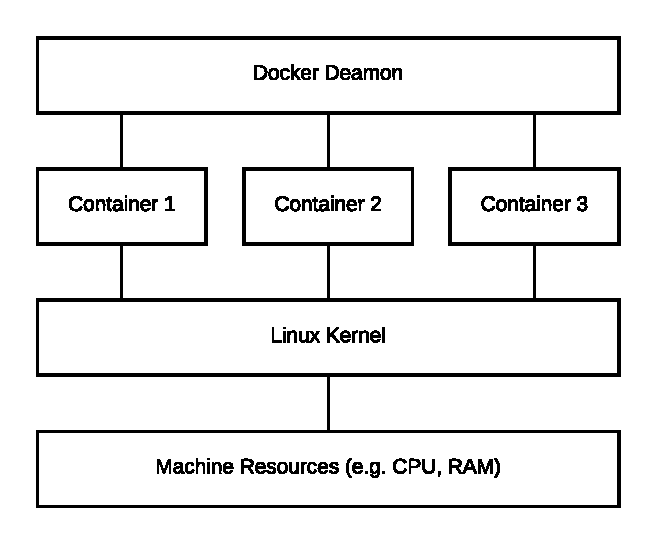
\includegraphics[scale=1]{images/04_technical_background/docker/container_structure}
\caption{Docker basic container structure - Source: Authors own model, based on \cite{Bullington2020Docker}.}
\label{fig:04_docker_container_container-structure}
\end{figure}

% Container advantages
The advantage of a container is its lightweight nature. As illustrated in \Fig{fig:04_docker_container_container-structure}, containers take advantage of OS-level virtualization instead of hardware-virtualization without the need of a hypervisor \cite{Docker2020Docs, Nickoloff2019Docker}. Containers share the resources of the host-system instead of using reserved resources \cite{Bullington2020Docker}. Multiple containers can run on the host-system kernel and are by default isolated from each other \cite{Docker2020Docs}.
% Docker container
In Docker, a container is a runnable unit of an image and is used for distributing and testing applications. A container can be configured to expose certain resources to the host system, e.g. network ports \cite{Bullington2020Docker}.


\subsection{Docker Swarm Mode}
\label{subsec:04_docker_swarm}
% What is Docker swarm
Docker Swarm mode is the native cluster orchestration and management tool embedded in the Docker engine.
% What is a swarm
In Docker Swarm mode, a cluster of multiple nodes is called a swarm. All nodes run in Swarm mode and act as managers or workers.
% Whats the purpose
In a swarm, multiple services can be deployed. The manager node is responsible to maintain the desired state of a service \cite{Docker2020Docs}.


% 
Many properties of Docker Swarm mode contribute the fact that it is an ideal tool to create self-healing and self-adapting environment:
\begin{itemize}
\item Desired state: The manager node monitors the state of each service in the swarm and adapts the environment to maintain the desired state \cite{Docker2020Docs}.

\item Cluster management and orchestration: Docker Swarm mode is integrated within the Docker engine. A swarm can be created and managed using the Docker CLI \cite{Docker2020Docs}.

\item Service model: The Docker engine allows to define the desired state of a service. The manager node maintains the desired state of all services in the swarm \cite{Docker2020Docs}.

\item Scaling: The number of replicas can be defined for each service. The manager node will automatically adapt the number of replicas for a service to keep the desired state \cite{Docker2020Docs}.

\item Multi-host networking: A swarm runs all services in an overlay network. New services will automatically be added to the overlay network \cite{Docker2020Docs}.
\end{itemize}


\subsubsection{Nodes}
% What is a node
A Docker engine participating in the swarm is called a node.
% What about the node role
Nodes can act as manager nodes, worker nodes or both \cite{Docker2020Docs}.


% What about the manager
The manager node is responsible for cluster orchestration an management. It maintains the desired state of all services and tasks in the swarm. In addition, the manager node dispatches tasks to worker nodes when service definitions will be submitted to the manager node \cite{Docker2020Docs}.


% What about worker
Worker nodes are responsible to execute the tasks receives by the manager node. While performing the tasks, the worker node notifies the manager node about the tasks state \cite{Docker2020Docs}.


\subsubsection{Services and Tasks}
% What is a service
A services defines the desired state of a task. The state is defined by the number of replicas of a service and the configuration for the Docker container, e.g. Docker Image, resources, network, and more \cite{Docker2020Docs}.


%What is a node
A task is a running Docker container. The task is defined by the corresponding service and will be managed by the manager node. A task can be performed on worker and manager nodes \cite{Docker2020Docs}.


% ===========================================
% ===========================================
% Apache Spark
% ===========================================
% ===========================================
\section{Apache Spark}
\label{sec:04_spark}
Apache Spark is an open-source computing framework for parallel data processing on a large computer cluster. Apache Spark manages the available resources and distributes computation tasks across a cluster to perform big-data processing operations at large scale \cite{Chambers2018Spark}. Before Apache Spark was developed, Hadoop MapReduce \cite{Dean2010MapReduce} was the framework of choice for parallel operations on a computer cluster \cite{Zaharia2010Spark}. Spark accomplished to outperform Hadoop by 10x for iterative Machine Learning \cite{Zaharia2010Spark}. It is implemented in Scala\footnote{The Scala programming language - \url{https://www.scala-lang.org/} (Accessed: 2020-12-18)}, a JVM-based language and provides a programming interface for Scala, Java\footnote{Java Software - \url{https://www.oracle.com/java/} (Accessed: 2020-12-18)}, Python\footnote{Python programming language - \url{https://www.python.org/} (Accessed: 2020-12-18)}, and R\footnote{The R Project for Statistical Computing - \url{https://www.r-project.org/} (Accessed: 2020-12-18)}. Additionally, Apache Spark includes an interactive SQL shell and libraries to implement Machine Learning and streaming applications \cite{Chambers2018Spark}.


\subsection{Spark Programming Model}
\label{subsec:04_spark_pr-model}
% Explain RDDs
Apache Spark provides resilient distributed datasets (RDDs) as the main abstraction for parallel operations \cite{Zaharia2010Spark}. Core types of the higher-level structured API are built on top of RDDs and will automatically be optimized by the Catalyst optimizer to run operations quick and efficient \cite{Chambers2018Spark, Hien2018Spark}.


\subsubsection{Resilient distributed datasets}
% What are RDDs
Resilient distributed datasets are fault-tolerant, parallel data structures to enable data sharing across cluster applications \cite{Zaharia2012RDDs}. They allow to express different cluster programming models like MapReduce, SQL and batched stream processing \cite{Zaharia2012RDDs}. RDDs have been implemented in Apache Spark and serve as the underlying data structure for higher level APIs (Spark structured API) \cite{Zaharia2012RDDs}.
% How can RDDs be used in applications
RDDs are a immutable, partitioned collection of records and can only be initiated through transformations (e.g. map, filter) on data or other RDDs.
% What are the advantages of RDDs
An advantage of RDDs is, that they can be recovered through lineage. Lost partitions of an RDD can be recomputed from other RDDs in parallel on different nodes \cite{Zaharia2012RDDs}. 
% Better use structured API
RDDs are lower level APIs and should only be used in applications if custom data partitioning is needed \cite{Chambers2018Spark}. It is recommended to use Sparks structured API objects instead. Optimizations for RDDs have to be implemented manually while Apache Spark automatically optimizes the execution for structured API operations \cite{Chambers2018Spark}.


\subsubsection{Apache Spark Structured API}
% What is the structured API
Apache Spark provides high level structured APIs for manipulating all kinds of data. The three distributed core types are Datasets, DataFrames and SQL Tables and Views \cite{Chambers2018Spark}.
% About DataFrames, Datasets and SQL
Datasets and DataFrames are immutable, lazy evaluated collections that provide execution plans for operations \cite{Chambers2018Spark}. SQL Tables and Views work the same way as DataFrames, except that SQL is used as the interface instead of using the DataFrame programming interface \cite{Chambers2018Spark}.
% Differences between Datasets ad Dataframes
Datasets use JVM types and are therefore only available for JVM based languages. DataFrames are Datasets of type \texttt{Row}, which is the optimized format for computations \cite{Chambers2018Spark}.


\subsubsection{Apache Spark Catalyst}
\label{subsubsec:04_spark_pr-model_catalyst}
% What is the Catalyst optimizer
Apache Spark also provides a query optimizer engine called Apache Spark Catalyst. \Fig{fig:04_spark_pr-model_catalyst_process} illustrates how the Spark Catalyst optimizer automatically optimizes Apache Spark applications to run quickly and efficient.
% Short How
Before executing the users code, the Catalyst optimizer translates the data-processing logic into a logical plan and optimizes the plan using heuristics \cite{Hien2018Spark}. After that, the Catalyst optimizer converts the logical plan into a physical plan to create code that can be executed \cite{Hien2018Spark}.


% What are logical plans
Logical plans get created from a DataFrame or a SQL query. A logical plan represents the data-processing logic as a tree of operators and expressions where the Catalyst optimizer can apply sets of rule-based and cost-based optimizations \cite{Hien2018Spark}.
For example, the Catalyst can position a filter transformation in front of a join operation \cite{Hien2018Spark}.

% What are physical plans
From the logical plan, the Catalyst optimizer creates one ore more physical plans which consist of RDD operations \cite{Chambers2018Spark}. The cheapest physical plan will be generated into Java bytecode for execution across the cluster \cite{Hien2018Spark}.

% Spark Catalyst figure
\begin{figure}[h]
\centering
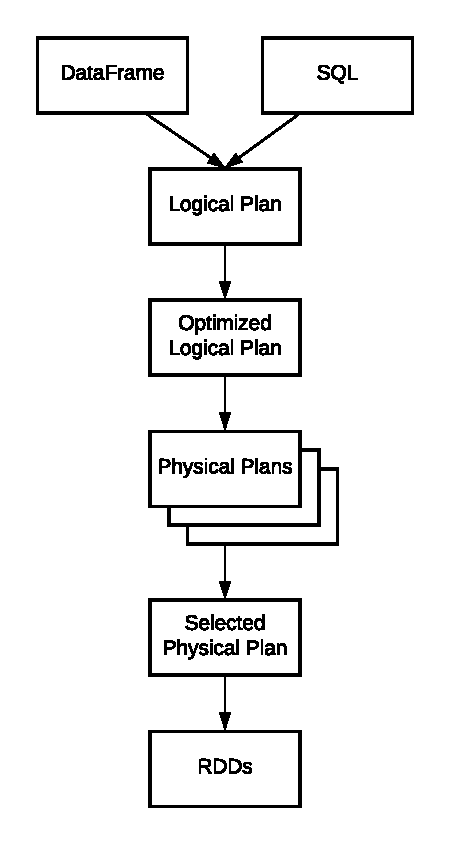
\includegraphics[scale=1]{images/04_technical_background/spark/catalyst_optimization_process}
\caption{Optimization process of the Spark Catalyst - Source: Authors own model, based on \cite{Hien2018Spark}.}
\label{fig:04_spark_pr-model_catalyst_process}
\end{figure}


\subsection{Application Architecture}
\label{subsec:04_spark_architecture}

\begin{figure}[h]
\centering
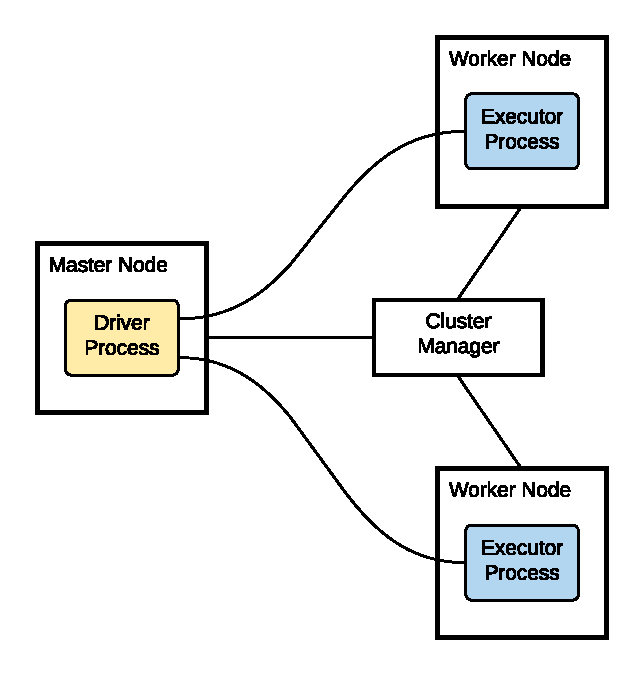
\includegraphics[scale=1]{images/04_technical_background/spark/spark_cluster_architecture}
\caption{Overview of a Spark cluster architecture - Source: Authors own model, based on \cite{Apache2020Spark}.}
\label{fig:spark_cluster_overview}
\end{figure}

% Explain image
\Fig{fig:spark_cluster_overview} illustrates the main architecture of an Apache Spark cluster running an application.
% Master-Worker
The architecture follows the master-worker model.
% The processes
Each running application has one driver process (master) and multiple executor processes (worker) exclusively assigned by the cluster manager.
% Cluster manager
Furthermore, the cluster manager decides on which nodes the processes will be executed \cite{Hien2018Spark}.


\subsubsection{Driver Process}
\label{subsubsec:04_spark_architecture_driver}
The driver process is a JVM process running on a physical machine and responsible to maintain the execution of an Apache Spark application \cite{Chambers2018Spark}. It coordinates the application tasks onto each available executor \cite{Hien2018Spark}. 
The driver interacts with the cluster manager to launch executors and allocate hardware resources \cite{Chambers2018Spark, Hien2018Spark}.


\subsubsection{Executor Process}
% JVM
The executor process is a JVM process, that runs through the whole duration of an application \cite{Hien2018Spark, Apache2020Spark}.
% Tasks
It is responsible to perform all tasks (units of work) assigned by the driver process \cite{Chambers2018Spark}.
% Report
After the executor process finish, it reports back to the driver process \cite{Chambers2018Spark}.
% CPU
Each task will be performed on a separate CPU core to enable parallel processing \cite{Hien2018Spark}.


\subsubsection{Cluster Manager}
\label{subsubsec:04_spark_architecture_manager}
The cluster manager is an external service that orchestrates the work between available machines in the cluster \cite{Hien2018Spark, Apache2020Spark}.
% Worker and master nodes
It decides on which nodes in the cluster the driver process and the executor processes will be launched.
% Resources
Additionally, the cluster manager manages the resources of each node in the cluster \cite{Hien2018Spark, Chambers2018Spark}.
% Different cluster types
Apache Spark supports different services that can run as cluster manager: Standalone mode (introduced in \Sec{subsec:04_spark_standalone}), Apache Mesos\footnote{Apache Mesos - \url{https://mesos.apache.org/} (Accessed: 2021-01-02)}, Hadoop YARN\cite{Murthy2013Yarn}, and Kubernetes\footnote{Kubernetes - \url{https://kubernetes.io/} (Accessed: 2021-01-02)} \cite{Apache2020Spark}.
% Explain different cluster deploy modes
The cluster manager provides three different deploy modes for acquiring resources in the cluster.
\begin{itemize}
% Cluster mode
\item Cluster mode:
To run an application in cluster mode, the user has to submit a precompiled JAR, python script or R script to the cluster manager \cite{Chambers2018Spark}. After that, the cluster manager starts the driver process and executor processes exclusively for the Apache Spark application on machines inside the cluster \cite{Chambers2018Spark, Hien2018Spark}.

% Client mode
\item Client mode:
The difference between the client mode and the cluster mode is that, the driver process runs on the client machine outside of the Spark cluster \cite{Chambers2018Spark}.

% Local mode
\item Local mode:
The local mode starts an Apache Spark application on a single computer \cite{Chambers2018Spark}. It is important to mention, that the local mode is not recommended to use in production. Instead it should be used for testing Apache Spark applications \cite{Chambers2018Spark}.
\end{itemize}


\subsection{Standalone Cluster Deployment}
\label{subsec:04_spark_standalone}
% What is a standalone cluster
The standalone mode is a basic cluster-manager build specifically for Apache Spark. It is developed to only run Apache Spark but supports workloads at large scale \cite{Chambers2018Spark}.
% Why standalone cluster mode, advantages


\subsubsection{Starting Master and Worker Nodes}
\paragraph{}Apache Spark provides executable launch scripts to start master and worker nodes in standalone mode.
% Where to find them
The executables can be found at \texttt{sbin/start-master.sh} to start a master node and at \texttt{/start-slave.sh} to start a worker node.
% parameter for worker script
The worker launch executable requires the master node URI as parameter \cite{Apache2020Spark}. 


% Example master
\begin{lstlisting}[label=lst:04_spark_standalone_launch-master, caption=Usage of master launch script, language=bash]
$ ./sbin/start-master.sh
\end{lstlisting}


% Example worker
\begin{lstlisting}[label=lst:04_spark_standalone_launch-worker, caption=Usage of worker launch script, language=bash]
$ ./sbin/start-slave.sh spark://spark-master:7077
\end{lstlisting}


% Introduce examples
\paragraph{}\Lst{lst:04_spark_standalone_launch-master} and \Lst{lst:04_spark_standalone_launch-worker} provide an example of how to use both executables to start a master and a worker node. The URI \texttt{spark://spark-master:7077} in \Lst{lst:04_spark_standalone_launch-worker} is an example of a master node URI. The master node launch script will print out the master URI after being executed successfully \cite{Apache2020Spark}.


\subsubsection{Resource Allocation}
\label{subsubsec:04_spark_standalone_res-alloc}
In standalone mode, worker need a set of resources configured. Therefore, a worker can assign resources to executors.
% Discovery script
To specify how a worker discovers resources, a discovery script has to be available \cite{Apache2020Spark}.


\subsubsection{Submitting Applications with spark-submit}
\label{subsubsec:04_spark_standalone_submit}
% Which executable
\paragraph{}To submit an application to a standalone cluster, Apache Spark provides the \texttt{spark-submit} executable. The executable file is available at \texttt{bin/spark-submit} in the installation folder of Apache Spark.
% Cluster mode
In cluster mode the driver of an Apache Spark application (see \Sec{subsubsec:04_spark_architecture_driver}) will be launched from one of the worker processes inside the cluster.
% When does it finish
The submit process will finish after it has submitted the application. It does not wait for the submitted application to finish \cite{Apache2020Spark}.


% Example
\begin{lstlisting}[label=lst:04_spark_standalone_submit_example, caption=Example usage of the spark-submit executable, language=bash]
$ bin/spark-submit --master spark://spark-master:7077 application.py
\end{lstlisting}


% How to use it
\paragraph{}\Lst{lst:04_spark_standalone_submit_example} shows how the spark-submit executable can be used to submit a Python application to a standalone Apache Spark cluster.
% required parameter
Spark-submit requires the master node URI and the path to the desired Spark application file.
% Which files
With the spark-submit executable it is possible to submit Python, Java and R applications \cite{Apache2020Spark}.


% ===========================================
% ===========================================
% NVIDIA RAPIDS
% ===========================================
% ===========================================
\section{RAPIDS accelerator for Apache Spark}
\label{sec:04_rapids}
% Explain
RAPIDS accelerator for Apache Spark is a plugin suite that aims to accelerate computing operations for Apache Spark using GPUs. It is available for Apache Spark 3 \cite{SparkRapids2020Docs}.
% A little how
The plugin uses the RAPIDS\footnote{Open GPU Data Science - \url{https://rapids.ai/} (Accessed: 2021-01-01)} libraries to extend the Apache Spark programming model, introduced in \SubSec{subsec:04_spark_pr-model} \cite{SparkRapids2020Docs, Mcdonald2020SparkRapids}.


\subsection{Extension of the Spark programming model}
\label{subsec:04_rapids_ext}
% How does it extends DataFrame and SQL
\paragraph{}The plugin suite extends the Apache Spark programming model with a new DataFrame based on Apache Arrow\footnote{Arrow. A cross-language development platform for in-memory data - \url{https://arrow.apache.org/} (Accessed: 2020-12-03)} data structures. In addition, the Catalyst optimizer (described in \SubSec{subsubsec:04_spark_pr-model_catalyst}) is extended to generate GPU-aware query plans \cite{Mcdonald2020SparkRapids}.
% What is Apache Arrow
Apache arrow is a data platform to build high performance applications that work with large datasets and to improve analytic algorithms. A component of Apache Arrow is the Arrow Columnar Format, an in-memory data structure specification for efficient analytic operations on GPUs and CPUs \cite{ApacheArrow2020Docs}.


% RAPIDS query plan image
\begin{figure}[h]
\centering
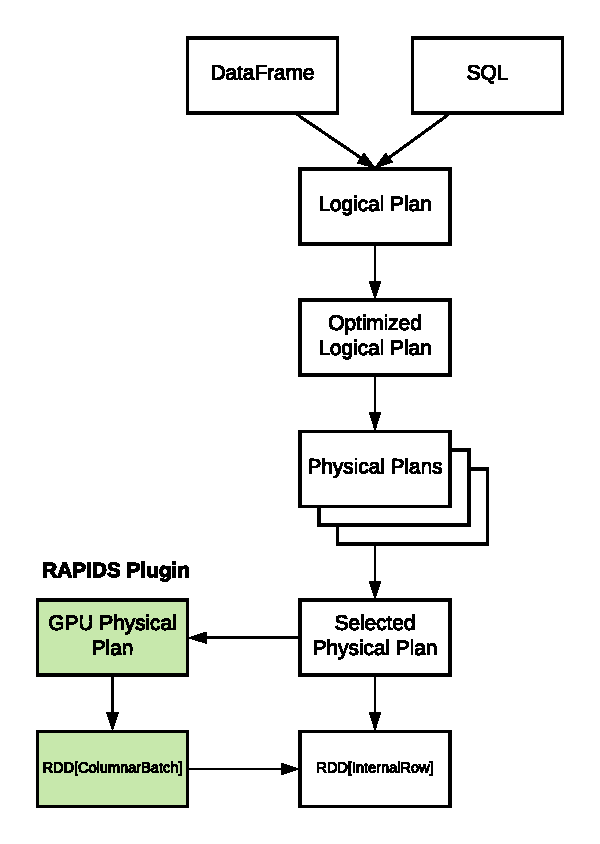
\includegraphics[scale=1]{images/04_technical_background/rapids/rapids_catalyst_optimization_process}
\caption{Catalyst optimization with RAPIDS accelerator for Apache Spark - Source: Authors own model, based on \cite{Mcdonald2020SparkRapids}.}
\label{fig:04_rapids_ext_query-plan}
\end{figure}
\paragraph{}\Fig{fig:04_rapids_ext_query-plan} illustrates how the RAPIDS plugin suite extends the Catalyst optimization process illustrated previously in \Fig{fig:04_spark_pr-model_catalyst_process}.
% How does the Catalyst create GPU aware plans
The Spark Catalyst optimizer identifies operators in a query plan that are supported by the RAPIDS API. To execute the query plan, these operators can be scheduled on a GPU within the Spark cluster \cite{Mcdonald2020SparkRapids}. If operators are not supported by the RAPIDS APIs, a physical plan for CPUs will be generated by the Catalyst optimizer to execute RDD operations \cite{Mcdonald2020SparkRapids}.


\subsection{Installation Requirements for Apache Spark Standalone Mode}
\label{subsec:04_rapids_req}
The RAPIDS accelerator for Apache Spark is available for a standalone mode Apache Spark cluster. To operate effectively, the following requirements need to be installed on all Apache Spark nodes in the cluster \cite{SparkRapids2020Docs}:
% requirements
\begin{itemize}
\item Java Runtime Environment (JRE)
\item NVIDIA GPU driver
\item CUDA Toolkit\footnote{CUDA Toolkit - \url{https://developer.nvidia.com/cuda-toolkit} (Accessed: 2021-01-01)}
\item RAPIDS accelerator for Apache Spark Java library
\item cudf Java library which is supported by the RAPIDS accelerator Java library and the installed CUDA toolkit
\item GPU resource discovery script
\end{itemize}


% ===========================================
% ===========================================
% PROMETHEUS
% ===========================================
% ===========================================
\section{Prometheus}
\label{sec:04_prom}
% What is Prometheus
Prometheus is an open-source monitoring and alerting system \cite{Prom2020Docs}.
% Time-series format + PromQL
To collect and store data, Prometheus supports a multi-dimensional key-value pair based data model, according to \SubSec{subsec:02_monitoring_db_multi-metrics}, which can be analyzed in using the PromQL query language \cite{Pandey2020Monitoring}.
% SHort PromQL
PromQL is a functional query language for selecting and aggregating time-series data in real-time \cite{Prom2020Docs}.
% Pull-based approach
Prometheus follows the pull-based approach, as described in detail in \SubSec{subsec:02_monitoring_push-pull}, to scrape metrics from hosts and services \cite{Bastos2019Prom}.


\subsection{Prometheus Architecture}
% Architecture image
\begin{figure}[h]
\centering
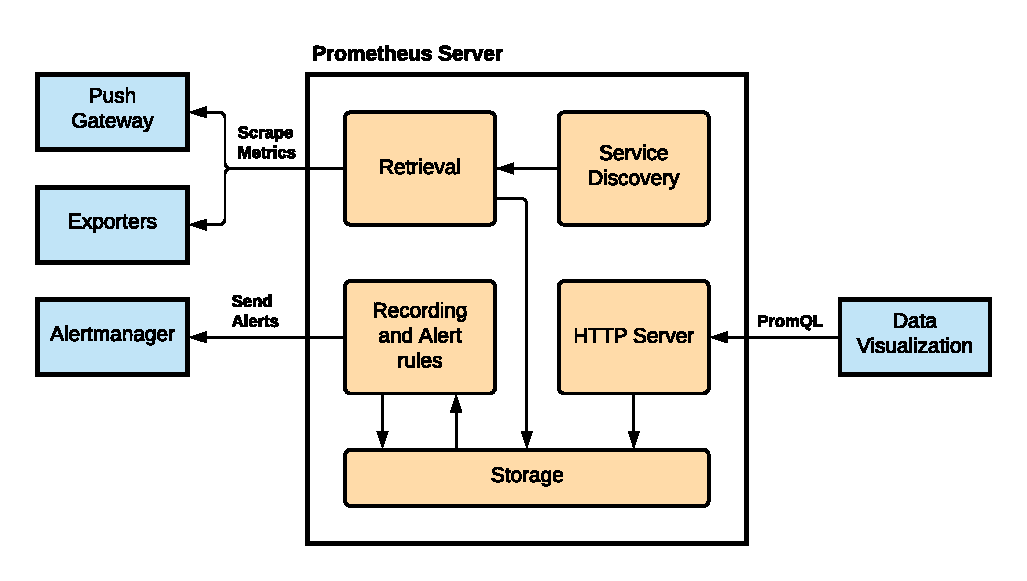
\includegraphics[scale=0.8]{images/04_technical_background/prometheus/prometheus_architecture}
\caption{Prometheus high-level architecture - Source: Authors own model, based on \cite{Prom2020Docs, Brazil2018Prom}.}
\label{fig:prom_architecture}
\end{figure}

% High level architecture
\Fig{fig:prom_architecture} illustrates the high-level architecture of Prometheus.
% Description of components
The Prometheus ecosystem provides multiple components. Components can be optional, depending on the monitoring needs of the environment \cite{Bastos2019Prom}. The main components of a Prometheus system are Prometheus Server, Alertmanager, service discovery, exporters, Push Gateway, and data visualization \cite{Prom2020Docs}.

\subsubsection{Prometheus Server}
% SHort intro
The Prometheus server is the main component of a Prometheus system. It is responsible to collect metrics as time-series data from targets and stores the collected data in the built-in TSDB \cite{Bastos2019Prom}. Prometheus uses the concept of scraping to collect metrics from a target. A target host has to expose an endpoint to make metrics available in the Prometheus data format \cite{Pandey2020Monitoring}. Additionally, the Prometheus server triggers alerts to the Alertmanager if a configured condition becomes true \cite{Prom2020Docs}.
% The figure
The core components of the Prometheus Server, as illustrated in \Fig{fig:prom_architecture}, are the following:

\begin{itemize}
% Service discovery
\item Service Discovery:
As being mentioned before, Prometheus follows a pull-based approach to fetch metrics from a target. To know about all targets, Prometheus needs a list of the corresponding hosts. The service discovery manages the complexity of maintaining a list of hosts manually in an changing infrastructure \cite{Bastos2019Prom}. Therefore, Prometheus is able to notice targets which are not responding \cite{Brazil2018Prom}.

% Retrieval
\item Retrieval:
Prometheus sends a HTTP request to each target to scrape metrics. The request is send each interval, which can be set in the configuration \cite{Brazil2018Prom}.

% HTTP API
\item HTTP API:
Prometheus provides a HTTP API. This API can be used to request raw data and evaluate PromQL queries.
Data visualisation tool can use this API to create visualisations of the requested metrics \cite{Brazil2018Prom}.

% Recording rules and alerts
\item Recording and alert rules:
Recording rules enable to precompute frequently needed or compute-intensive PromQL expressions. The result will be saved as a set of time-series in the local storage. This enables to query a recording rule at a much faster speed than the original PromQL expression \cite{Brazil2018Prom, Prom2020Docs}.

Alert rules define conditions based on PromQL expressions. If a condition becomes true, an alert will be send to an external service \cite{Prom2020Docs}.

% Storage
\item Storage:
Received data is stored in a custom highly efficient format on a local on-disk time-series database \cite{Prom2020Docs}. Prometheus does not offer a solution for distributed storage across a cluster of machines \cite{Brazil2018Prom}.
\end{itemize}


\subsubsection{Optional Components}
The Prometheus ecosystem offers a set of components which are optional and can be activated depending on the monitoring needs.
The optional components illustrated in \Fig{fig:prom_architecture} are the following:

\begin{itemize}
% Alertmanager
\item Alertmanager:
If an alerting rule becomes true, the Prometheus server generates an alert and pushes it to the Alertmanager. The Alertmanager generates notifications from the received alerts. A notification can take multiple forms like emails or chat messages. Webhooks can be implemented to trigger custom notifications \cite{Bastos2019Prom}.

% Exporters
\item Exporters:
If an application does not support an endpoint for Prometheus, an exporter can be used to fetch metrics and make them available to the Prometheus server. An exporter is a monitoring agent running on a target host that fetches metrics from the host and exports them to the Prometheus server \cite{Pandey2020Monitoring}.

% Push Gateway
\item Push Gateway:
If a target is not designed to be scraped, metrics can be pushed against the Push Gateway \cite{Prom2020Docs}. The Push Gateway converts the data into the Prometheus data format and passes them to the Prometheus server \cite{Pandey2020Monitoring}.

% Data vis
\item Data Visualisation:
Prometheus supports various tools for virtualization of the scraped data. Grafana\footnote{Grafana: The open observability platform - \url{https://grafana.com/} (Accessed: 2021-01-19)} is one of the widely used tools for this occasion.
\end{itemize}


\subsection{Prometheus Configuration}
% Short intro
Configuration related to scraping jobs and rules are configured in configuration files. Configuration are written in the YAML file format \cite{Prom2020Docs}.


% Explain listing
\Lst{lst:04_prom_config_example} shows a valid configuration file example.
% global section
In the \texttt{global} configuration section, default values can be set.
% scrape_configs
Targets are defined in the \texttt{scrape\_configs} section. Each target is defined as a scrape job with a unique name.  A target can be defined statically using the \texttt{static\_configs} parameter or dynamically using the available service discovery mechanisms \cite{Prom2020Docs}.
% rules
Rules have to be configured in a separate YAML file. To load rules into Prometheus, the file path has to be set in the \texttt{rule\_files} parameter.

% config file example
\begin{lstlisting}[label=lst:04_prom_config_example, caption=Prometheus configuration file example]
global:
  scrape_interval: 5s

scrape_configs:
  - job_name: cadvisor
    static_configs:
      - targets: ["cadvisor:8080"]
        labels:
          group: "cadvisor"
          
rule_files:
  - "/etc/prometheus/recording_rules.yml"
\end{lstlisting}

% rules example
\Lst{lst:04_prom_config_rule-example} is an configuration example of a recording rule.
% Rule config
Rules are defined in a rule group. Each rule is defined by a name and a valid PromQL expression \cite{Prom2020Docs}.

% Recording rule example
\begin{lstlisting}[label=lst:04_prom_config_rule-example, caption=Prometheus rules configuration file example]
groups:
  - name: http_requests
     - record: job:http_inprogress_requests:sum
        expr: sum by (job) (http_inprogress_requests)
\end{lstlisting}


% ===========================================
% ===========================================
% CADVISOR
% ===========================================
% ===========================================
\section{cAdvisor}
% What is cAdvisor
Container Advisor (cAdvisor) is a running deamon that collects, aggregates, analyses and exposes performance metrics from running containers.
% How to run
It has native support for Docker container and is deployed as a Docker container.
% How it collects
cAdvisor collects metrics from the container deamon and Linux cgroups.
% How it exposes
Collected metrics will be exposed in the Prometheus file format \cite{Bastos2019Prom, cadvisor2020Docs}.


% ===========================================
% ===========================================
% Gitlab CI/CD
% ===========================================
% ===========================================
\section{GitLab CI/CD}
\label{sec:04_background_gitlab}
GitLab CI/CD is a tool integrated into the GitLab platform that enables Continuous Integration (CI), Continuous Delivery (CD) and Continuous Deployment (CD) for software development.
% Gitlab platform
The GitLab platform integrates many development features like Git repository management and CI/CD.
% How it works
By pushing code changes to the codebase, GitLab CI/CD executes a pipeline of scripts to automate CI and CD processes of the software development cycle.
% CI
A CI pipeline will consist of scripts that builds, tests and validate the updated codebase.
% CD
A CD pipeline is responsible to deploy the application for production after the CI pipeline has executed successfully.
% Summary
Adding CI/CD pipelines to the software development cycle of an application, allows to catch bugs an errors early. This ensures that an application deployed to production will conform to established standards \cite{Gitlab2020Docs}.

\subsection{CI/CD Pipeline}

The fundamental component of GitLab CI/CD is called a pipeline. Pipelines will perform based on conditions. A conditions might be a push to the main branch of the repository \cite{Gitlab2020Docs}. A pipeline comprises two components:

\begin{itemize}
\item Stages: A stage consists of one or multiple jobs that run in parallel. Furthermore, a stage defines how jobs will be executed. For example, a build stage only performs after a test stage has performed successfully \cite{Gitlab2020Docs}.

\item Jobs: Jobs are responsible to perform the scripts defined by administrators. The scripts define necessary actions. For example compiling the source code or performing tests \cite{Gitlab2020Docs}.
\end{itemize}


% How to configurate a pipeline (.gitlab-ci.yml)
GitLab CI/CD is configured by a \texttt{.gitlab-ci.yml} file. It is necessary that this file is located in the repositories root directory.
% What does this file
The configuration file will create a pipeline that performs after a push to the repository \cite{Gitlab2020Docs}.


\subsection{Example of a Basic CI/CD Pipeline Architecture}

\begin{figure}[h]
\centering
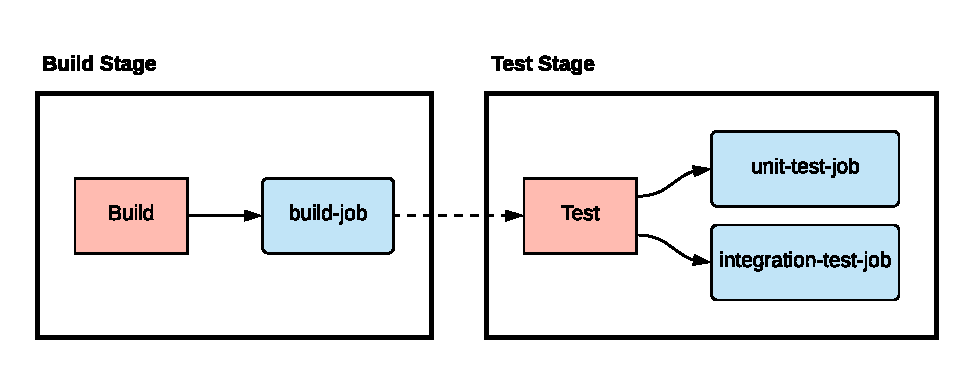
\includegraphics[scale=0.8]{images/04_technical_background/gitlab/basic_pipeline}
\caption{Basic architecture of a GitLab CI/CD pipeline - Source: Authors own model, based on \cite{Gitlab2020Docs}.}
\label{fig:04_gitlab_pipeline_basic_arch}
\end{figure}

% Explain figure
\Fig{fig:04_gitlab_pipeline_basic_arch} illustrates an architecture of a basic CI/CD pipeline.
% Two stages
The pipeline consists of a build and a test stage. Stages will be performed in order. The test stage will only be performed after the build stage was successful.
% Build stage
The build stage consists of a single job named \textit{build\_job}. This job is executed first, after a change is pushed to the repository.
% Test stage
Two jobs exist in the test stage. These jobs are executed in parallel when the test stage is triggered.


% Example config

% Explain example
\Lst{lst:04_gitlab_pipeline_basic_config-example} provides the configuration for the basic pipeline example.
% Shell script
Each job executes a shell script to perform the desired actions. The shell scripts have to be located in the source code repository.
% The example
\begin{lstlisting}[label=lst:04_gitlab_pipeline_basic_config-example, caption=Example of a \texttt{.gitlab-ci.yml} configuration file]
stages:
  - build
  - test

build-job:
  stage: build
  script:
    - build_software.sh

unit-test-job:
  stage: test
  script:
    - run_unit_tests.sh
    
integration-test-job:
  stage: test
  script:
    - run_integration_tests.sh
\end{lstlisting}


\subsection{Job Execution}
% Runner pick up jobs
Jobs which are defined in the configuration file will be performed by GitLab runners.
% What is runner
A GitLab runner is an agent that performs the jobs in its own environment and responds the result back to the GitLab instance. A runner is a lightweight and highly scalable application that runs on a server and performs one or multiple executors.
% WHat is an executor
An executor provides the environment where jobs will be executed in. GitLab runner provides multiple variants of executors.
% The docker executor
For example the Docker executor that connects to the underlying Docker engine. In addition, the Docker executor performs a job in a separate and isolated Docker container.
% Runner config
GitLab runner can be set up only for specific projects or be available to all project on the GitLab platform \cite{Gitlab2020Docs}.


% ===========================================
% ===========================================
% Scaling heat
% ===========================================
% ===========================================
\section{Scaling Heat}
\label{sec:04_scal-heat}
% Intro
The Scaling Heat algorithm is a decision making algorithm to determine if a scaling action is necessary.
% Authors and why
It was introduced by Barna et al. \cite{Barna2017ElasticContainerApps} to overcome issues of traditional recurrence factor algorithms \cite{Barna2017ElasticContainerApps}.


\subsection{Recurrence Factor}
% Why recurrence factor
\paragraph{}In an Autonomic Computing environment, a scaling decision is made in each interval after data has been retrieved from the monitoring system (see \Sec{sec:02_ac} for the Autonomic Computing architecture). 
% Performance spikes
Sudden performance spikes can occur and can cause the decision algorithm to perform unnecessary scaling actions.
% The problem
These unnecessary scaling actions can have a negative impact on the overall computing performance.
% The recurrence factor
To overcome this issue, a recurrence factor needs to be introduced to the decision making algorithm.
% What it does
With a recurrence factor ($n$), a scaling action will only be performed until a performance threshold has been violated $n$ times \cite{Barna2017ElasticContainerApps}.


% Problems of traditional recurrence factor algos
\paragraph{}Traditional recurrence factor algorithm require violations to occur regularly. If a performance violation of the opposite direction occurs, the algorithm can get stuck in the violation process. Therefore, no scaling actions will be performed \cite{Barna2017ElasticContainerApps}.


\subsection{Scaling Heat Algorithm Concept}
\label{sec:04_background_scaling-heat}
% The algorithm
\begin{algorithm}[H]
\SetKwInput{KwInput}{Input}
\SetKwInput{KwOutput}{Output}
\SetAlgoLined
\KwInput{$utilization$ - The retrieved utilization for a performance metric}
\KwInput{$lower\_threshold$ and $upper\_threshold$ - Range limit of the performance metric}
\KwInput{$heat$ - Current heat value of a performance metric. Indicating if a scaling action is necessary}
\KwOutput{$heat$ - New heat value for the next iteration}
\uIf{$utilization \geq upper\_threshold$}{
   \tcp{cluster overload}
   \uIf{$heat < 0$}{
     \tcp{reset heat for removal}
     $heat \leftarrow 0$\;
   }
   $heat \leftarrow heat + 1$\;
   }
   \uElseIf{$utilization \leq lower\_threshold$}{
     \tcp{cluster overload}
     \uIf{$heat > 0$}{
       \tcp{reset heat for adding}
       $heat \leftarrow 0$\;
     }
     $heat \leftarrow heat - 1$\;
   }  
   \Else{
   \tcp{utilization is within threshold range}
   \tcp{move heat towards 0}
   \uIf{$heat > 0$}{
      $heat \leftarrow heat - 1$\;
   }
   \uElseIf{$heat < 0$}{
      $heat \leftarrow heat + 1$\;   
   }
  }
\uIf{$heat = n$}{
Perform a scale-out action\;
$heat \leftarrow 0$\;
}
\uElseIf{$heat = -n$}{
Perform a scale-in action\;
$heat \leftarrow 0$\;
}
\Return{heat}
\caption{Scaling Heat decision making algorithm\cite{Barna2017ElasticContainerApps}}
\label{alg:04_scal-heat_concept_algo}
\end{algorithm}


% Describe the concept
\paragraph{}\Alg{alg:04_scal-heat_concept_algo} introduces the Scaling Heat algorithm.
% The base
The algorithm is based in a concept called \textit{heat}. The value of heat indicates if a scaling action of removing or adding components is necessary.
% Violations
If the given utilization of a performance metric violates the upper threshold, the heat value will increase. Violations of the lower threshold will cause a decrease respectively.
% Recurrence
When the heat reaches the recurrence factor $n$, positive for adding and negative for removing nodes, a scaling action will be executed.
% Reset
After executing a scaling action, the heat value will be set to 0 \cite{Barna2017ElasticContainerApps}.


% ===========================================
% ===========================================
% KHP
% ===========================================
% ===========================================
\section{Kubernetes Horizontal Pod Autoscaler}
\label{sec:04_background_khpa}
\paragraph{}
% Short intro
Kubernetes Horizontal Pod Autoscaler (KHPA) is an auto-scaling algorithm used in Kubernetes.
% Pod?
Kubernetes is an orchestration tool that allows to create and deploy units called Pods. A Pod is a running process on a cluster that encapsulates an application.
% What
KHPA scales the number of replicas per Pod based on the utilization of performance metrics.
% Interval
The algorithm is based on a control loop. Each $n$ seconds, the algorithm gathers performance metrics and computes the target number of replicas to achieve the desired utilization of a performance metric \cite{Casalicchio2017AutoScaleCont}.


% Support for multiple metrics
The algorithm computes the number of replicas for a single performance metric. If a scaling action depends on multiple performance metrics, the number of replicas has to be computed for each performance metric. The largest number of replicas is used as the target number of replicas \cite{Kubernetes2021Docs}.


\paragraph{}
KHPA takes as input the number of active replicas for a pod ($active\_replicas$), the utilization of the performance metric of each replica ($pod\_utilization$), and the target utilization of the performance metric ($target\_utilization$).
% Intro formula
The formula to compute the target number of pods $P$ is defined by \cite{Kubernetes2021Docs}:
% The formula
\begin{equation}
P = \left \lceil active\_replicas \times \left ( \frac{\sum pod\_utilization}{target\_utilization} \right ) \right \rceil
\label{eq:04_background_khpa_equation}
\end{equation}

